\Level 0 {Vector graphics and raster graphics}

We may use fancy techniques such as Bezier curves for describing
shapes, but at some point the graphic needs to be rendered on an actual
device with pixels or ink dots. Thus we need algorithms for deciding
which pixels to turn on or off, and, in case the device has a larger
bitdepth, with what intensity.

The technical terms here are `\index{vector graphics}vector graphics'
for a description of the lines and curves, and
`\index{raster graphics}raster graphics' for the pixel-by-pixel
description.
A~description of a raster is also called `\index{bitmap}bitmap'.
Common bitmap-based formats are JPEG, GIF, TIFF, PNG, PICT, and BMP.

Vector graphics make for a much more compact file, but they rely on
the presence of a final rendering stage. For instance, Macromedia's
Flash format (now an open Internet standard) is a vector graphics
format, that relies on a browser plugin. However, presence of a Flash
renderer is pretty much standard in browsers these days.
Adobe Postscript is also a vector format. The first popular printer to
incorporate it, the Apple Laserwriter, had a Motorola 68000 processor,
exactly as powerful as the Macintosh computer it connected to.

Two vector standards are being proposed to the W3C: the Precision
Graphics Markup Language and the Vector Markup Language. PGML is
backed by Adobe Systems, IBM, Netscape, and Sun Microsystems. VML is
supported by Microsoft, Hewlett-Packard, Autodesk, Macromedia, and
Visio. Both standards are based on Extensible Markup Language (XML).

\Level 0 {Basic raster graphics}

\Level 1 {Line drawing}

We limit the discussion to lines with slope less than~1. For those, on
a grid of pixels, one pixel per column will be switched on, and the
question to be addressed is which pixel to turn on in each column.
\begin{figure}
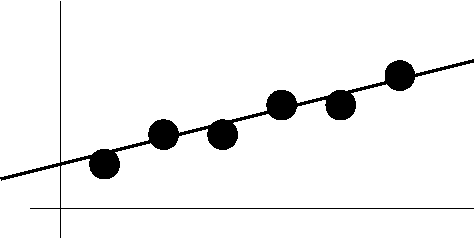
\includegraphics[scale=.5]{one-per-column}
\caption{Line with slope~$\leq1$ and one pixel per column on}
\end{figure}

Probably the simplest way to draw a line is by using an
`\index{incremental drawing}incremental' drawing algorithm. Let a line
$y=mx+B$ be given, and we write the slope as~$m=\delta y/\delta x$. In
the case of pixel graphics, we set~$\delta x\equiv1$, so $\delta y=m$
and we can
recursively state \[y_{i+1}=y_i+\delta y.\]
The simplest implementation of this is
\begin{quote}
\begin{tabbing}
let $x_0,y_0$ and $m$ be given, then\\
for \=$i=0\ldots n-1$\\
\>\n{WritePixel}$(x_i,\mathop{\textrm{Round}}(y_i))$\\
\>$x_{i+1}=x_i+1$\\
\>$y_{i+1}=y_i+m$
\end{tabbing}
\end{quote}
Since  $(x_i,y_i)$ is never related to the actual formula for the line,
there will be an accumulation of round-off error. However, this will
be negligible. More seriously, the rounding operation is relatively
expensive. In the next algorithm we will eliminate it. If possible, we
want to operate completely in integer quantities.

\begin{figure}
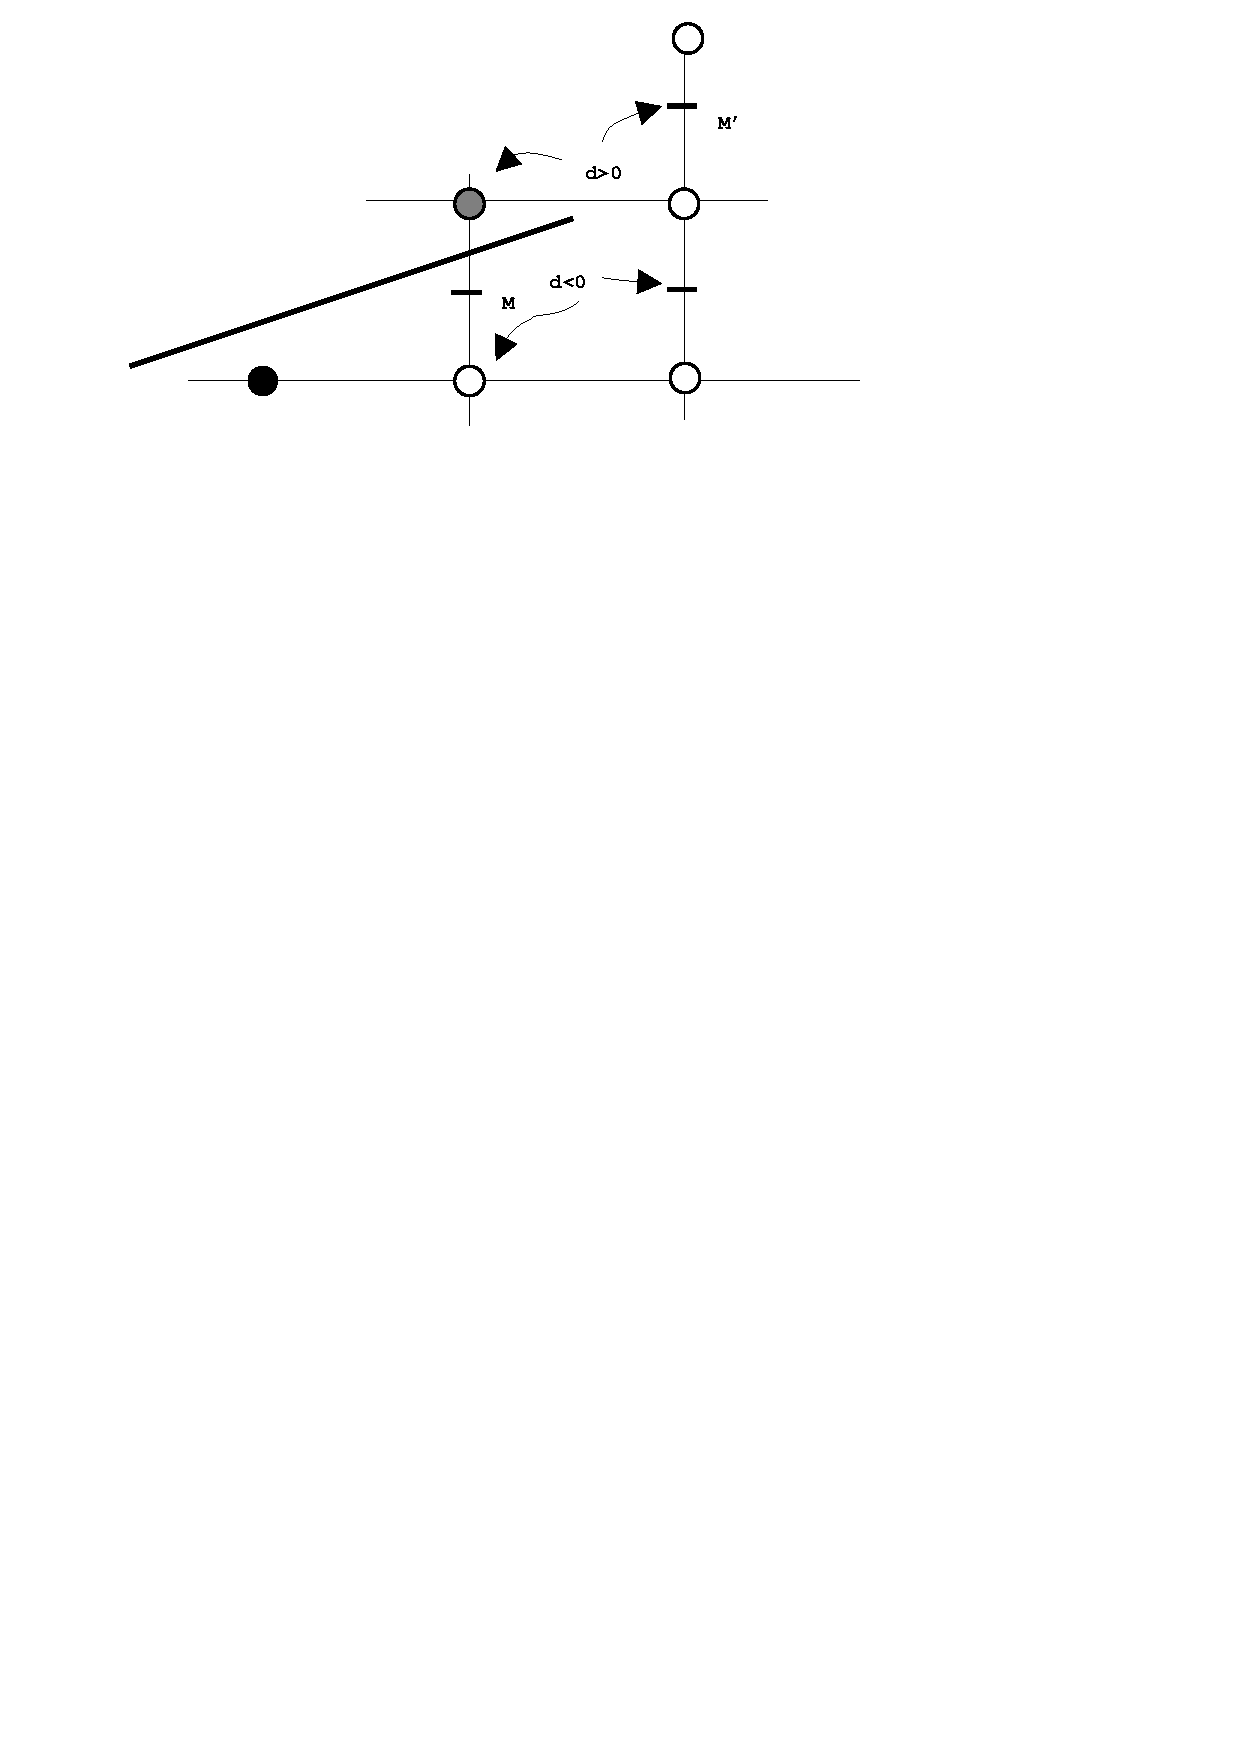
\includegraphics[scale=.7]{line-midpoint}
\caption{The midpoint algorithm for line drawing}
\end{figure}

The `midpoint algorithm' proceeds fully by integer addition. First we
write the equation for the line in two different ways as
\[ y={dy\over dx}x+B, \qquad F(x,y)=ax+by+c=0.\]
Clearly, $a=dy$, $b=-dx$, $c=B$, and we can derive $dx,dy$ from the
end pixels of the line. The function~$F$ is zero on the line, positive
in the half plane under it, and negative above it.

Now we consider how to progress given that we have switched on a pixel
at~$(x_p,y_p)$. With the initial assumption that the line has a slope
between 0~and~1, the next pixel will be either $(x_P+1,y_P+1)$, or
$(x_p+1,y_p)$, depending on which is closer to the line. 

Instead of measuring the distance of the candidate next pixels to the
line, we decide whether their midpoint~$M$ is above or under the line. For
this, we use the function~$F(\cdot,\cdot)$ introduced above, and
evaluate the `decision value' of the midpoint:
\[ d=F(x_p+1,y_p+1/2). \]
The two cases to consider then are
\begin{description}
\item[$d<0$:] $M$ lies over the line, so we take $y_{p+1}=y_p$;
\item[$d\geq0$:] $M$ lies under the line, so we take $y_{p+1}=y_p+1$.
\end{description}
Similarly we update the mid point: if $d\geq0$, the midpoint moves up.
Note that the new midpoint is at $x_{p+1}+1$.

Now, we do not actually use the midpoint, only the value of~$d$.
The algorithm is then complete once we find a way to update~$d$ cheaply.
For this we look at its next value
\[ d'=F(x_{p+1}+1,y_{p+1}+1/2). \]
Corresponding to the above two cases:
\[ \begin{array}{rll}
    d'=&a(x_{p+1}+1)+b(y_{p+1}+1/2)+c=\\
    d<0:&= a(x_p+2)+b(y_p+1/2)&=d+a=d+dy\\
    d\geq0:&= a(x_p+2)+b(y_p+3/2)+c&=d+a+b=d+dy-dx
\end{array} \]
In other words, we update~$d$ with $dy$ or~$dy-dx$ depending on
whether it's negative or non-negative.

To start off the algorithm, $dx$~and~$dy$ are computed from the
endpoints, and the initial value of~$d$ follows from
\[ d_0=F(x_0+1,y_0+1/2)=F(x_0,y_0)+a+b/2=0+dy-dx/2.\]
To get rid of the division by~2, which would cause real rather than
integer values to be used throughout the algorithm,
we can redefine $\tilde
F(x,y)=2F(x,y)$; correspondingly we update~$d$ with $2dy$
and~$2(dy-dx)$ in the two cases.
\begin{594exercise}
Can you modify the DDA line drawing algorithm so that it works (as
well as possible) when the line is given between points that are not
on pixels?
\end{594exercise}
\begin{answer}
If the begin point has real coordinates, round the $x$~coordinate to a
pixel, and approximate the $y$~coordinate as~$n/m$ with fairly small
integers~$m,n$. By scaling the function~$F$ by~$m$ all the
calculations become integer again.
\end{answer}

These algorithms are sometimes referred to as `\index{DDA}Digital
Differential Analyzers', since they trace out a curve by proceeding
with small differences. The line algorithm was first derived by Bressenham.

\Level 1 {Circle drawing}

Circles can be drawn with a similar algorithm. We observe that,
because of 8-fold symmetry, we can limit the algorithm to the part of
a circle from $x=0$ to~$x=y$. The midpoint argument is now slightly
more complicated. The function for the circle is 
\[ F(x,y) = x^2+y^2-R^2,\]
and the decision value in the midpoint~$M$ is 
\[ d=F(x_p+1,y_p+1/2)=x^2+2x+y^2+y+5/4. \]

\begin{figure}
\includegraphics[scale=.7]{circle-midpoint}
\caption{The midpoint algorithm for circle drawing}
\end{figure}

The two cases to consider are similar to before:
\begin{description}
\item[$d<0$:] $M$ lies in the circle, so we take $y_{p+1}=y_p$;
\item[$d\geq0$:] $M$ lies outside the circle, so we take $y_{p+1}=y_p+1$.
\end{description}
To update the decision value we get the two cases
\[ \begin{array}{rll}
    d'=&F(x_{p+1}+1,y_{p+1}+1/2)=\\
    d<0:&= x^2+4x+y^2+y+4\,1/4&=d+2x+3\\
    d\geq0:&= x^2+4x+y^2+3y+6\,1/4&=d+2(x+y)+5
\end{array} \]
\begin{594exercise}
Why is there no need to consider bigger increments of~$y_p$ in the
circle drawing algorithm? After all, a~circle has curvature so the
slope increases.
\end{594exercise}
\begin{answer}
Since the algorithm considers only an octant, the slope is never more
than~1.
\end{answer}

The circle algorithm can be further improved by observing that the
quantities $2x$ and~$2y$ can themselves easily by constructed by
updating. This removes the need for any multiplication.

\Level 1 {Cubics}

Suppose we have a cubic function $f(t)=at^3+bt^2+ct+d$. Instead
of evaluating this polynomial directly, using Horner's rule, we
compute the value $f(t+\delta)$ by updating:
\[ f(t+\delta)=f(t)+\Delta f(t). \]
We find 
\[ \begin{array}{rcl}
    \Delta f(t)&=&f(t+\delta)-f(t)\\
        &=&a(3t^2\delta+3t\delta^2+\delta^3)+b(2t\delta+\delta^2)+c\delta\\
        &=&3a\delta
    t^2+(3a\delta^2+2b\delta)t+a\delta^3+b\delta^2+c\delta
\end{array} \]
This still leaves us with a quadratic function to evaluate, so we
define 
\[ \begin{array}{rcl}
    \Delta^2f(t)&=&\Delta f(t+\delta)-\Delta f(t)\\
        &=&3a\delta(2t\delta+\delta^2)+(3a\delta^2+3b\delta)\delta\\
        &=&6a\delta^2t+6a\delta^3+2b\delta^2
\end{array} \]
Finally, we derive
$\Delta^3f(t)=\Delta^2f(t+\delta)-\Delta^2f(t)=6a\delta^2$. Taken all
together, we can now compute $f_{n+1}\equiv f((n+1)\delta)$ by
initializing
\[ \Delta^3f_0=6a\delta^2,\quad
    \Delta^2f_0=6a\delta^3+2b\delta^2,\quad
    \Delta f_0=a\delta^3+b\delta^2+c\delta
\]
and computing by update
\[  f_{n+1}=f_n+\Delta f_n,\quad
    \Delta f_{n+1}=\Delta f_n+\Delta^2f_n,\quad
    \Delta^2f_{n+1}=\Delta^2f_n+\Delta^3f_0
\]
The advantage of this algorithm is its low operation count, and the
fact that it works fully by integer operations.

\Level 0 {Rasterizing type}

Typefaces can be described by curves, but several aspects to them make
it necessary to do more than just rendering these curves, when
rasterizing them. Part of the problem is that characters in a font are
relatively small, and satisfy all sorts of constraints that both may be
hard to satisfy (especially at low resolution), and are immediately
noticed when rendered incorrectly.
\begin{figure}[ht]
\includegraphics[scale=.75]{raster-problems}
\includegraphics[scale=.75]{illegible}
\caption{Problems in rasterizing type, and resulting illegible output}
\end{figure}

Such problems result from using too simple algorithms for converting
the character outlines to rasters.
\begin{figure}[ht]
\includegraphics[scale=.75]{e-bad}
\includegraphics[scale=.75]{e-good}
\caption{A bad and a good way of rendering a Times Roman `e' at low
  resolution}
\label{fig:e-pimple}
\end{figure}
For instance, an obvious algorithm is
\begin{quote}
A pixel is turned on if its center is within the curve.
\end{quote}
Now consider the case where a curve with large radius exceeds location
$y=n+1/2$ for only one~$x$. This results in the `pimple' on top of the
`e' in figure~\ref{fig:e-pimple}. On the other hand, if such a curve
stays just under such a halfpoint, we get a long plateau, as in the
left side curve of the~`e'.

\Level 1 {Scaled fonts}

These rasterizing problems are largely due to the facts that
\begin{itemize}
\item Characters are scalable, so the relations between top/bottom or
  left/right are not always mapped the same way to a pixel grid;
\item Even if characters are used at the same size, they need to be
  displayed on various kinds of rasters (printer, screen);
\item Characters can be placed in any horizontal or vertical location,
  so relations to pixel boundaries are also flexible.
\end{itemize}

The conversion process goes more or less as follows\footnote{Much of
  this discussion is based on the definition of TrueType fonts.}:
\begin{figure}[ht]
\includegraphics[scale=.45]{fig2-1-1}
\includegraphics[scale=.45]{fig2-1-2}
\includegraphics[scale=.45]{fig2-1-3}
\includegraphics[scale=.45]{fig2-1-4}
\caption{Scaled and rasterized character outline}
\label{fig:raster-H}
\end{figure}
\begin{itemize}
\item Character outlines are based on coordinates on some grid, often
  expressed as fixed point, or other scheme with a finite mesh size.
\item The character is scaled to the raster on which it will be
  rendered.
\item The result is rounded to the raster, in
  figure~\ref{fig:raster-H} this puts the left and right sides on
  pixel boundaries; note that other vertical parts of the character
  are not necessarily pixel-aligned.
\item The scaled and rounded outline is then rasterized by turning a
  set of pixels on.
\end{itemize}
We see that in both final steps, rounding to the raster, and switching
on pixels, we can have unwanted effects.

\Level 1 {Pixelation}

Above we said that pixels are switched on if their center falls within
the curve. There are two problems with this:
\begin{itemize}
\item Sometimes not enough pixels are turned on to render the shape
  accurately, and
\item Deciding whether a pixel is within the shape is not trivial to
  begin with. For instance, letters such as `o' or `p' have an inner
  region that should not be filled. In another example, sometimes it
  is convenient to describe a shape as non-disjoint union of other
  shapes; see figure~\ref{fig:q=l+o}
\end{itemize}
\begin{figure}[ht]
\includegraphics[scale=.7]{overlapping-contours}
\caption{A shape consisting of overlapping contours}
\label{fig:q=l+o}
\end{figure}
The second problem can be solved a number of ways. We could for
instance look at a scan line, and switch to on/off mode every time we
cross a curve boundary. This approach does not work for intersecting
curves.

\begin{figure}[ht]
\includegraphics[scale=.7]{windingrules}
\caption{The effects of different winding number rules}
\label{fig:winding-number}
\end{figure}
Better solutions are based on looking at the so-called `winding
number'. This number counts, for a given point in the plane, how often
a curve winds around the point. If this is zero, the point is outside
the curve, otherwise it is inside it.

That implementing winding number rules is not trivial can be seen from
two screen shots of Acrobat Reader version~4;
figure~\ref{fig:AR4-winding}.
\begin{figure}
\includegraphics[width=5in]{winding_ar4win_100}\par
\includegraphics[width=5in]{winding_ar4win_150}
\caption{Acrobat 4 rendering of a complicated figure at different
  magnifications}
\label{fig:AR4-winding}
\end{figure}

\Level 1 {Font hinting / instructing}

\begin{figure}[ht]
\includegraphics[scale=.6]{o-horizontal}
\includegraphics[scale=.6]{o-vertical}
\caption{Constraints on the letter `O'}
\label{fig:o-constraints}
\end{figure}
To prevent some of the problems indicated above, characters in a font
file consist of more than just the outline description. Additionally,
each character can have a short program in a language defined by the
font file format. Such a program can enforce that certain distances
in the font as exact multiples of pixel distances.

For instance, the letter `O' in figure~\ref{fig:o-constraints} has the
following constraints
\begin{enumerate}
\item A certain amount of white space buffering the character;
  distance~3 is the `transport';
\item The width of the band
\item[5,6] Visual under and overshoot.
\item[7] The height of the band
\end{enumerate}
Distances 5 and~6 are over and undershoot: a letter with curved
top/bottom like~`O' would seem too small if it stayed between the
baseline and the cap height. To compensate for that, the letter is
made slightly higher and deeper. However, for small sizes and low
resolutions, this compensation needs to be switched off, since it
would look too drastic.

\Level 1 {Dropouts}

In certain cases, pixels can not be switched on that are necessary for
continuity of the figure drawn. Figure~\ref{fig:dropout} shows a case
where a connecting bit is too thin to hit the centers of any pixels.
\begin{figure}[ht]
\includegraphics[scale=.5]{dropout.pdf}
\caption{A case of `dropout': missing pixels give a disconnected curve}
\label{fig:dropout}
\end{figure}
To cover such cases, the renderer usually has an algorithm that
detects when a scan line enters and leaves a contour without setting
any pixels. It will then set, for instance, the left pixel.

\Level 0 {Anti-aliasing}

In the algorithms so far, the decision was between switching a pixel
on or off. There are a few problems with this. For instance, for
certain slopes the rendered curve can have a very `jagged' look. Also,
a curve at slope~1 will have the same number of pixels on as a curve
at slope~0, but on a path that is longer by~$\sqrt{2}$. Thus, it may
look lighter or thinner.

If the display supports a range of values (`grayscale'), we can try to
use this and find a better visual rendering. First we will look at an
example, then briefly consider the general theory of this phenomenon.

\Level 1 {Raster graphics with larger bitdepths}

In the algorithms above, pixels close to a line or other curve were
switched on. If the display supports it, we can compute a
measurement of proximity of the pixel to the line, and set a
brightness based on that. There are various ways to implement
this. For instance, one could consider the line to have an area, and
to compute the intersection area of the line and the pixel box. Here
we will use a `\index{filter function}filter function'. The support of
this function will be larger than the pixel box.

We will modify the midpoint method for line drawing so that in each
column three pixels will be nonzero, with an intensity based on the
Euclidean distance to the line. Let~$v$ be the (signed) vertical
distance from the midpoint to the line, and $D$~the euclidean
distance, then $D=vdx/\sqrt{dx^2+dy^2}$. The denominator we can
compute once and for all at the start of the algorithm, but a simple
way of computing~$vdx$ is needed.

Consider the case where~$d<0$, in which case we
choose~$y_{p+1}=y_p$. Now we have
\[ 0=F(x_p+1,y_p+v)=F(x_p+1,y_p)+2bv\Rightarrow 2vdx=F(x_p+1,y_p), \]
and
\[ d = F(M)=F(x_p+1,y_p+1/2)=F(x_p+1,y_p)+b \]
so $2vdx=d+dx$. Likewise, if~$d\geq0$, $2vdx=d-dx$. Since we know how
to update~$d$ cheaply, we can now iteratively compute~$D$.

For the top and bottom point, $D=2(1-v)dx/\sqrt{\ldots}$ and
$D=\nobreak 2(1+v)/\sqrt{\ldots}$, respectively.

\Level 1 {The general idea}

Smoothing out a picture with grayscales is usually called
`\index{anti-aliasing}anti-aliasing'. To see why, consider how the
parts of a graphics system fit together. After we derive a curve
or other two-dimensional object (this could be a projected surface) to
display, the exact values are sampled according to the pixel
resolution. By computing a Fourier transform of these samples, we get
an impression of the visual `frequencies' in the picture.

If, instead of simply switching on pixels based on the sampled curve, we
compute pixel values so that sampling them reproduces the frequency
spectrum, we get a picture that looks closer to the intended one.

\endinput
\Level 0 {Raster graphics in \Metafont}

The basic problem of raster graphics is to take a curve
\[ \bar z=\bar z(t),\quad t=0\ldots n \]
and render it by turning on certain pixels on a raster graphics
device, be this a screen or a printer.

The simplest solution to this problem is to round the points along to
the path to the closest pixel: the point $(1.1,2.7)$ is rounded
to~$(1,3)$\footnote{We will use pixel-based coordinates throughout
  this chapter.}. We will never discretize a single (curved) line;
rather we are interested in rendering an outlined area between two
curves. The rounding algorithm is then equivalent to saying that a
pixel belongs to the digitized region if its center lies in the
original, undiscretized, region.

\begin{comment}
\begin{594exercise}
The second formulation of the pixel choosing algorithm is more
constructive. Argue this. How do you test whether a pixel lies in
between two curves?
\end{594exercise}
\begin{answer}
The first formulation requires the algorithm to follow the curve. This
involves an infinite number of points, so one would have to solve the
problem of taking a finite subset of those, and not skip any points.
In the second formulation, only a finite number of pixels has to be
investigated.\par
A~curve is defined as the points for which some function
satisfies~$F(t)=\nobreak0$. The points in between two curves then
satisfy $F_1(t)\geq0$, $F_2(t)<0$.
\end{answer}
\end{comment}

The rounding algorithm leads to `ambiguous points': the points with
one coordinate equal to~$n+1/2$. This can be solved by shifting each
point by~$(\epsilon,\delta)$, where $\epsilon$~and~$\delta$ are less
than the resolution of the coordinates, and~$\delta<\epsilon$. This
guarantees that a path will never touch a pixel center.

This shifting algorithm also helps with another problem. The path
$(t,t)$ touches the pixels at $(0,0)$ and~$(1,1)$, which are not
adjacent. With shifting, the path briefly rounds to~$(1,0)$.

Suppose a curve is nearly `flat', either horizontally or
vertically. If it briefly exceeds an~$n+1/2$ point, the rounding
algorithm will lead to an inelegant `pimple'. The only solution to
this is not to put the curve there in the first place. The easiest
algorithm is `if a curve is nearly horizontal, round its~$y$
coordinate to an integer; if it is nearly vertical, round its~$x$
coordinate likewise'.

Conceivably one could do something more sophisticated, knowing the
curvature, and whether the curve is convex or concave.


MT:53--55 about interpolation

MT:473--480 about bisecting angles

Metafont book chapter 24
